\label{fnt8.1.1-2}

\begin{wrapfigure}{R}{0.25\textwidth}
	\vspace{-37pt}
  	\centering
	\begin{center}
	\begin{tikzpicture}[thick,scale=0.9, every node/.style={transform shape},background rectangle/.style={fill=white}, show background rectangle]
		\node[inner sep=0pt,rotate=-20] (fingers) at (-.7,4.3) {
\includegraphics[width=2cm]{pinchedFingers.png}};
		\node at (0,0) {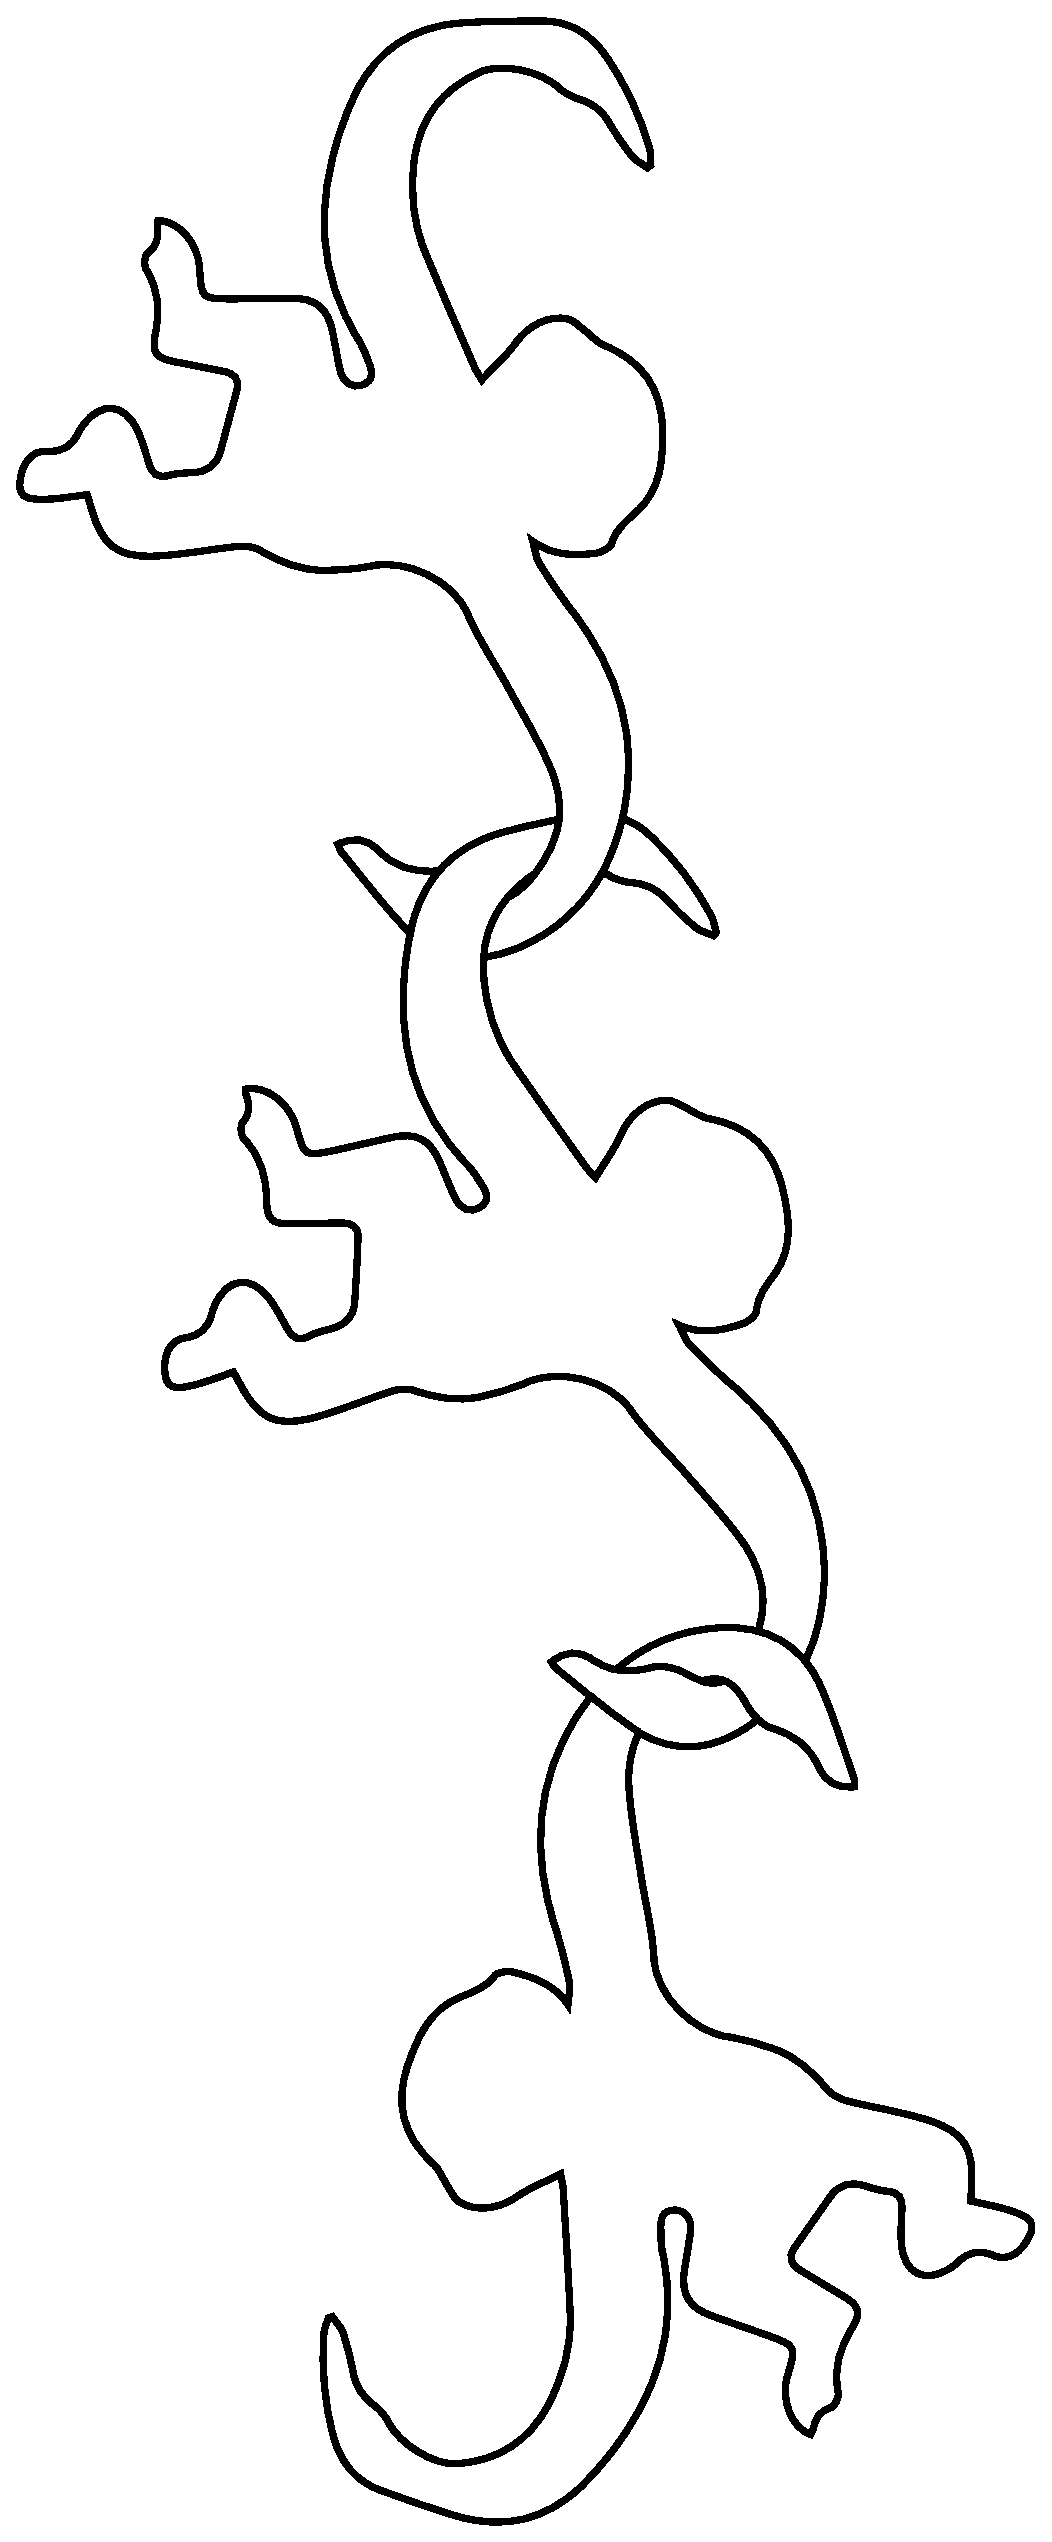
\includegraphics[width=3cm]{barrelmonkey.eps}};
		\node at (-0.25,2.4) {\scriptsize{$m=\unit[40]{g}$}};
		\node[rotate=2] at (0.12,0.1) {\scriptsize{$m=\unit[30]{g}$}};
		\node[rotate=-20] at (0.3,-2.5) {\scriptsize{$m=\unit[20]{g}$}};
	\end{tikzpicture}
	\vspace{20pt}
	\end{center}
\end{wrapfigure}

\noindent Your little brother is playing with monkeys in a barrel. The mass of each monkey is indicated in the illustration on the right. Note that your brother is holding the monkeys still and his hand weighs \unit[50]{N}.

\begin{enumerate}[(a)]
	\item Make a separate \forcediag{} for each of the four objects, the hand, top monkey, middle monkey, bottom monkey.
	
	\item Identify all 3rd law pairs of forces appearing in your \forcediags{} by circling the two forces and connecting them with a line.
	
	\item Use Newton's 1st and 3rd laws to numerically determine all of the forces acting on the monkeys and the hand. If necessary, redraw your \forcediags{}, so they are more to scale.
\end{enumerate}